% A role's pushdown configuration (state, stack) evolving over a depth-2 RecursiveCf run:
% the stack grows as the recursion descends (push on each `recurse`) and shrinks as it
% unwinds (pop on each `subresult`), ending EMPTY — the well-nested / Dyck-balanced
% acceptance condition. Palette: push=violet, pop=fuchsia, frame=violet, accept=green.
\documentclass[border=10pt]{standalone}
\usepackage{tikz}
\usepackage{amsmath}
\usepackage{amssymb}
\usepackage{xcolor}
\usetikzlibrary{positioning}
\definecolor{push}{HTML}{7C3AED}
\definecolor{pop}{HTML}{C026D3}
\definecolor{good}{HTML}{16A34A}
\definecolor{ink}{HTML}{1E293B}
\definecolor{slate}{HTML}{475569}
\begin{document}
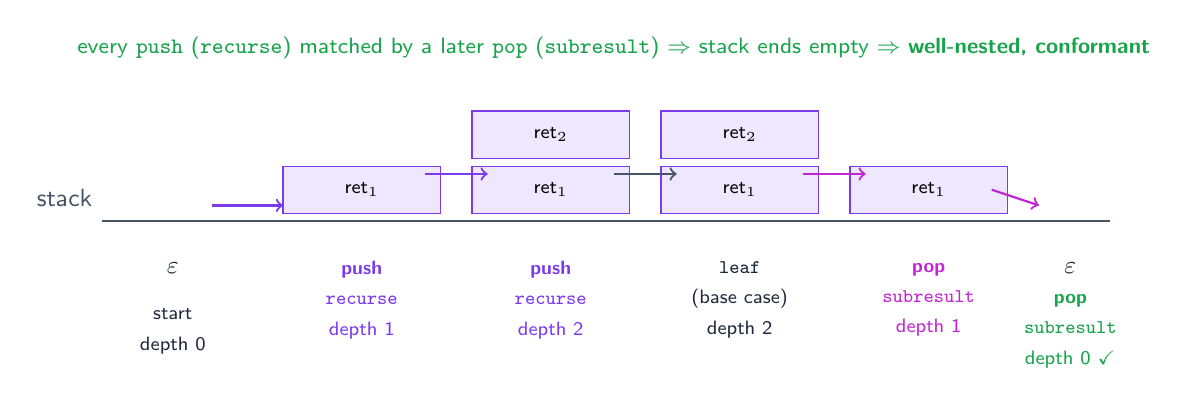
\begin{tikzpicture}[font=\sffamily\small,
    frame/.style={draw=push, fill=push!12, minimum width=20mm, minimum height=6mm, inner sep=1pt},
    base/.style={draw=slate, fill=slate!10, minimum width=20mm, minimum height=6mm, inner sep=1pt}]

  % baseline
  \draw[slate, thick] (-0.3,0) -- (12.5,0);
  \node[slate, left] at (-0.3,0.3) {stack};

  % step 0: empty
  \node[ink] at (0.6,-0.6) {$\varepsilon$};
  \node[ink, align=center] at (0.6,-1.4) {\scriptsize start\\\scriptsize depth 0};

  % step 1: push frame f1 (recurse, descend to level 1)
  \node[frame] (a1) at (3,0.4) {\scriptsize ret$_1$};
  \node[push, align=center] at (3,-1.0) {\scriptsize \textbf{push}\\\scriptsize \texttt{recurse}\\\scriptsize depth 1};

  % step 2: push frame f2 (recurse, descend to level 2 = bottom)
  \node[frame] (b1) at (5.4,0.4) {\scriptsize ret$_1$};
  \node[frame] (b2) at (5.4,1.1) {\scriptsize ret$_2$};
  \node[push, align=center] at (5.4,-1.0) {\scriptsize \textbf{push}\\\scriptsize \texttt{recurse}\\\scriptsize depth 2};

  % step 3: leaf base case — no stack change
  \node[frame] (c1) at (7.8,0.4) {\scriptsize ret$_1$};
  \node[frame] (c2) at (7.8,1.1) {\scriptsize ret$_2$};
  \node[ink, align=center] at (7.8,-1.0) {\scriptsize \texttt{leaf}\\\scriptsize (base case)\\\scriptsize depth 2};

  % step 4: pop frame (subresult unwind, level 2 -> 1)
  \node[frame] (d1) at (10.2,0.4) {\scriptsize ret$_1$};
  \node[pop, align=center] at (10.2,-1.0) {\scriptsize \textbf{pop}\\\scriptsize \texttt{subresult}\\\scriptsize depth 1};

  % step 5: pop frame (subresult unwind, level 1 -> 0) — EMPTY
  \node[ink] at (12,-0.6) {$\varepsilon$};
  \node[good, align=center] at (12,-1.4) {\scriptsize \textbf{pop}\\\scriptsize \texttt{subresult}\\\scriptsize depth 0 $\checkmark$};

  % arrows
  \draw[->, push, thick] (1.1,0.2) -- (2.0,0.2);
  \draw[->, push, thick] (3.8,0.6) -- (4.6,0.6);
  \draw[->, slate, thick] (6.2,0.6) -- (7.0,0.6);
  \draw[->, pop, thick] (8.6,0.6) -- (9.4,0.6);
  \draw[->, pop, thick] (11.0,0.4) -- (11.6,0.2);

  \node[good, align=center, font=\sffamily\footnotesize] at (6.2,2.2)
    {every \texttt{push} (\texttt{recurse}) matched by a later \texttt{pop} (\texttt{subresult}) $\Rightarrow$ stack ends empty $\Rightarrow$ \textbf{well-nested, conformant}};
\end{tikzpicture}
\end{document}
